%************************************************************
\section{Discrete-State Markov Chain}\label{app:markov_chain}
%************************************************************

This section of the appendix complements the most important theorems of Markov chain in relation to \gls[hyper=false]{mcmc} simulation presented in Section~\ref{sub:bc_mcmc_mc}.
In the following some of the important notions are first introduced for the discrete-state Markov chain.
It provides a more intuitive entry to the theory of Markov chain through matrix notation and a graphical representation.
The associated theorems are presented without proof though the list of references are provided.

% Markov Chain
A Markov chain on a discrete-state space $\mathcal{S}$ is defined as a sequence of random variables $\{\mathcal{X}^{(i)}; i \geq 0\}$ where the indices represents successive iterations,
\emph{such that the conditional probability distribution of $\mathcal{X}^{(i+1)}$ follows the Markov assumption}.
\marginpar{Markov chain}
That is,
\begin{equation}
  \mathcal{X}^{(i+1)}\,|\,\mathcal{X}^{(i)}, \mathcal{X}^{(i-1)}, \ldots, \mathcal{X}^{(0)} = \mathcal{X}^{(i+1)}\,|\,\mathcal{X}^{(i)}
\label{eq:app_markov_property}
\end{equation}
Put differently, the future value depends on the past only through the present value \cite{Geyer2011,Sokal1997}.

% Ingredients
A discrete-state Markov chain is fully defined by its joint probability \cite{Sokal1997}.
\begin{equation}
	\begin{split}
  \mathbb{P}(\mathcal{X}^{(i+1)} & = x^{(i+1)}, \mathcal{X}^{(i)} = x^{(i)}, \ldots, \mathcal{X}^{(0)} = x^{(0)}) = \\
	& \mathbb{P}(\mathcal{X}^{(0)} = x^{(0)}) \cdot \mathbb{P}(\mathcal{X}^{(1)} = x^{(1)}\,|\,\mathcal{X}^{(0)} = x^{(0)}) \cdot \ldots \\
	& \cdot \mathbb{P}(\mathcal{X}^{(i+1)}\,|\,\mathcal{X}^{(i)} = x^{(i)}) \cdot
	\end{split}
\label{eq:markov_chain_joint_probability}
\end{equation}
The specification consists of three main components:
\begin{itemize}

	\item The \emph{state space} $\mathcal{S}$ which is the set of all possible outcomes of the random variables $\{\mathcal{X}^{(i)}\}$.
	\marginpar{Discrete state space}
	The state space considered here is discrete with $D$ elements, $\mathcal{S} = \{x_1, x_2, \ldots, x_D \}$.
	
	\item The \emph{initial} probability distribution $\pi^{(0)}$.
	\marginpar{Initial distribution}
	This is the (marginal) probability distribution of $\mathcal{X}^{(0)}$ (or the marginal distribution of the chain at $i = 0$). That is,
	\begin{equation}
		\pi^{(0)} = \{\mathbb{P}(\mathcal{X}^{(0)} = x)\}  = \{\pi_x\} \,\,\, \forall x \in \mathcal{S}
	\label{eq:markov_chain_initial_distribution}
	\end{equation}
	In discrete-state Markov chain, the distribution can be expressed as a $D$-dimensional vector.
	
	\item The \emph{transition probability matrix} $P$ which is a $D \times D$ matrix with elements $p_{x,y} \geq 0.0$ and $\sum_y p_{x,y} = 1.0$.
	\marginpar{Transition probability}
	Each element is the conditional probability between two states. That is,
	\begin{equation}
		p_{x,y} = \mathbb{P}(\mathcal{X}^{(i+1)} = y | \mathcal{X}^{(i)} = x) \,\,\, \forall x,y \in \mathcal{S}
	\label{eq:markov_chain_transition_matrix_element}
	\end{equation}
	\marginpar{Stationary transition probability}
	The transition probability matrix is said to be \emph{stationary} if it does not depend on a particular iteration $i$.
	In practice, most \gls[hyper=false]{mcmc} algorithms rely on a stationary transition probability \cite{Geyer2011}.
\end{itemize}

% Example of Chain
As an example of a discrete-state Markov chain, consider a $3$-state Markov chain representing changes of human health condition with $\mathcal{S} = \{\text{Healthy}, \text{Sick}, \text{Dead}\}$ and a transition probability matrix $P$,
\begin{equation}
  P =  
    \begin{pmatrix}
      \mathbb{P}(H | H)  & \mathbb{P}(S | H) & \mathbb{P}(D | H)\\
      \mathbb{P}(H | S)  & \mathbb{P}(S | S) & \mathbb{P}(D | S)\\
      \mathbb{P}(H | D)  & \mathbb{P}(S | D) & \mathbb{P}(D | D)\\
    \end{pmatrix} =
		\begin{pmatrix}
		  0.75  & 0.20 & 0.05\\
      0.65  & 0.15 & 0.20\\
      0.00  & 0.00 & 1.00\\
		\end{pmatrix}
\label{eq:app_transition_probability_matrix}
\end{equation}
The Markov chain is graphically represented in Fig.~\ref{fig:app_markov_chain} using a \emph{state transition diagram}.
\begin{figure}[bth]
	\centering
	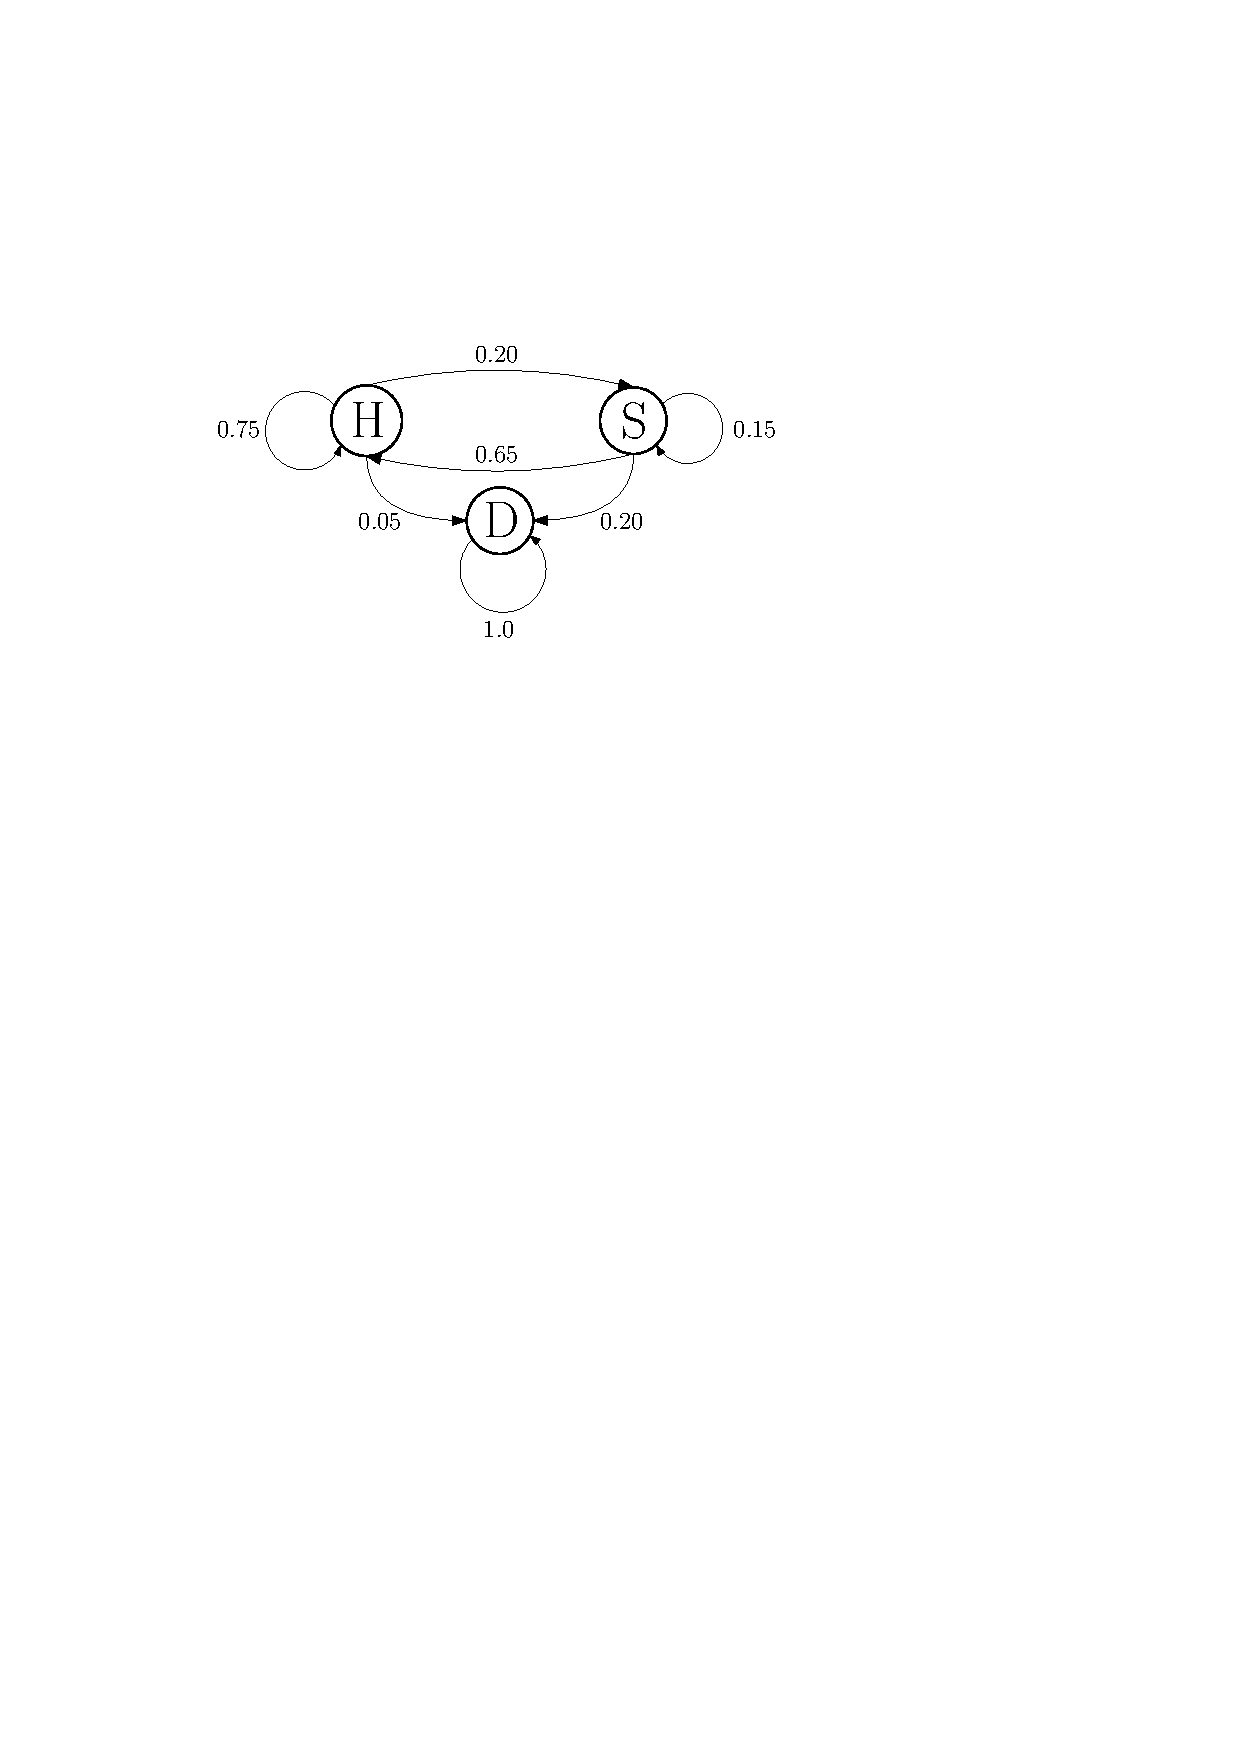
\includegraphics[width=0.9\textwidth]{../figures/chapter5/figures/markov_chain.pdf}
	\caption[Illustration of a $3$-State Markov Chain]{An illustration of a $3$-State Markov chain with the transition probability given by the matrix $P$ in Eq.~(\ref{eq:app_transition_probability_matrix}).}
	\label{fig:app_markov_chain}
\end{figure}

% Marginal Distribution at n-th transition
The probability of transition from state $x$ to $y$ in one iteration is given by,
\begin{equation}
	\begin{split}
		\mathbb{P}(\mathcal{X}^{(i+1)} = y) & = \sum_{x \in S} \mathbb{P}(\mathcal{X}^{(i)} = x) \cdot \mathbb{P}(\mathcal{X}^{(i+1)} = y | \mathcal{X}^{(i)} = x) \\
		\Leftrightarrow \pi^{(i+1)}_y  & = \sum_{x \in S} \pi_x^{(i)} \, p_{x,y}  \,\,\, \forall y \in \mathcal{S} \\
		\Leftrightarrow \pi^{(i+1)}    & = \pi^{(i)} \, P
	\end{split}
\label{eq:app_markov_chain_one_iteration}
\end{equation}
Thus, given the three main components, the marginal probability distribution at any given iteration can be defined recursively.
\marginpar{Marginal distribution of state at iteration $n$}
That is, the probability distribution at iteration $n$ is given by $\pi^{(n)} = \pi^{(0)} P^n$.
%Furthermore, the expression can be written in compact form as follows.
%For instance $1$-step transition from initial distribution $\pi^{(0)}$ by transition probability matrix $P$ yield the distribution,
%\begin{equation}
%	\pi^{(1)} = \pi^{(0)} P
%\label{eq:app_markov_chain_one_step}
%\end{equation}
%Where $\pi^{(1)}$ is the probability distribution of states at step $1$.
%In general,
%\begin{equation}
%	\begin{split}
%		\pi^{(2)} & = \pi^{(1)} P \\
%		          & \vdots \\
%		\pi^{(n)} & = \pi^{(n-1)} P \\
%		          & = \pi^{(0)} P^n\\
%	\end{split}
%\label{eq:app_markov_chain_one_step}
%\end{equation}
%where the $n$-th power of $P$ is called the $n$-step transition probability matrix \cite{Sokal1997}.
%\marginpar{$n$-step transition probability}
%In other words, the state at step $n$ is distributed as the $n$-times transition of the initial distribution.
%Moreover, due to the stationarity of the transition probability,
%this result also holds for an $n$-step transition of a distribution at any starting point,
%that is $\pi^{(i+n)} \thicksim \pi^{(i)} P^{(n)}$.  

% Irreducible Chain
A Markov chain is said to be \emph{irreducible} if each state in the state space $\mathcal{S}$ can be reached eventually from any other state \cite{Robert2004,Sargent2017}.
\marginpar{Irreducibility}
Irreducibility is a property of the transition probability matrix $P$ (i.e., having an irreducible transition probability matrix).
Formally,
\begin{equation}
	\forall x, y \in \mathcal{S}, \, \exists n \geq 0 \,\, \text{for which} \,\, p_{x,y}^{(n)} > 0
\label{eq:app_irreducibility}
\end{equation}
Based on this definition the transition matrix of Eq.~(\ref{eq:app_transition_probability_matrix}) is not irreducible as the state of being \emph{Dead} does not allow transition to any of the two other states.
An example of irreducible chain is given in a graphical representation of Fig.~\ref{fig:app_markov_chain_irreducible}.
Note that while state $B$ is not directly connected to state $A$,
the state can eventually be reached from state $B$ through the connection of state $C$ (in this case, $n$ is equal to $2$).
\begin{figure}[bth]
	\centering
	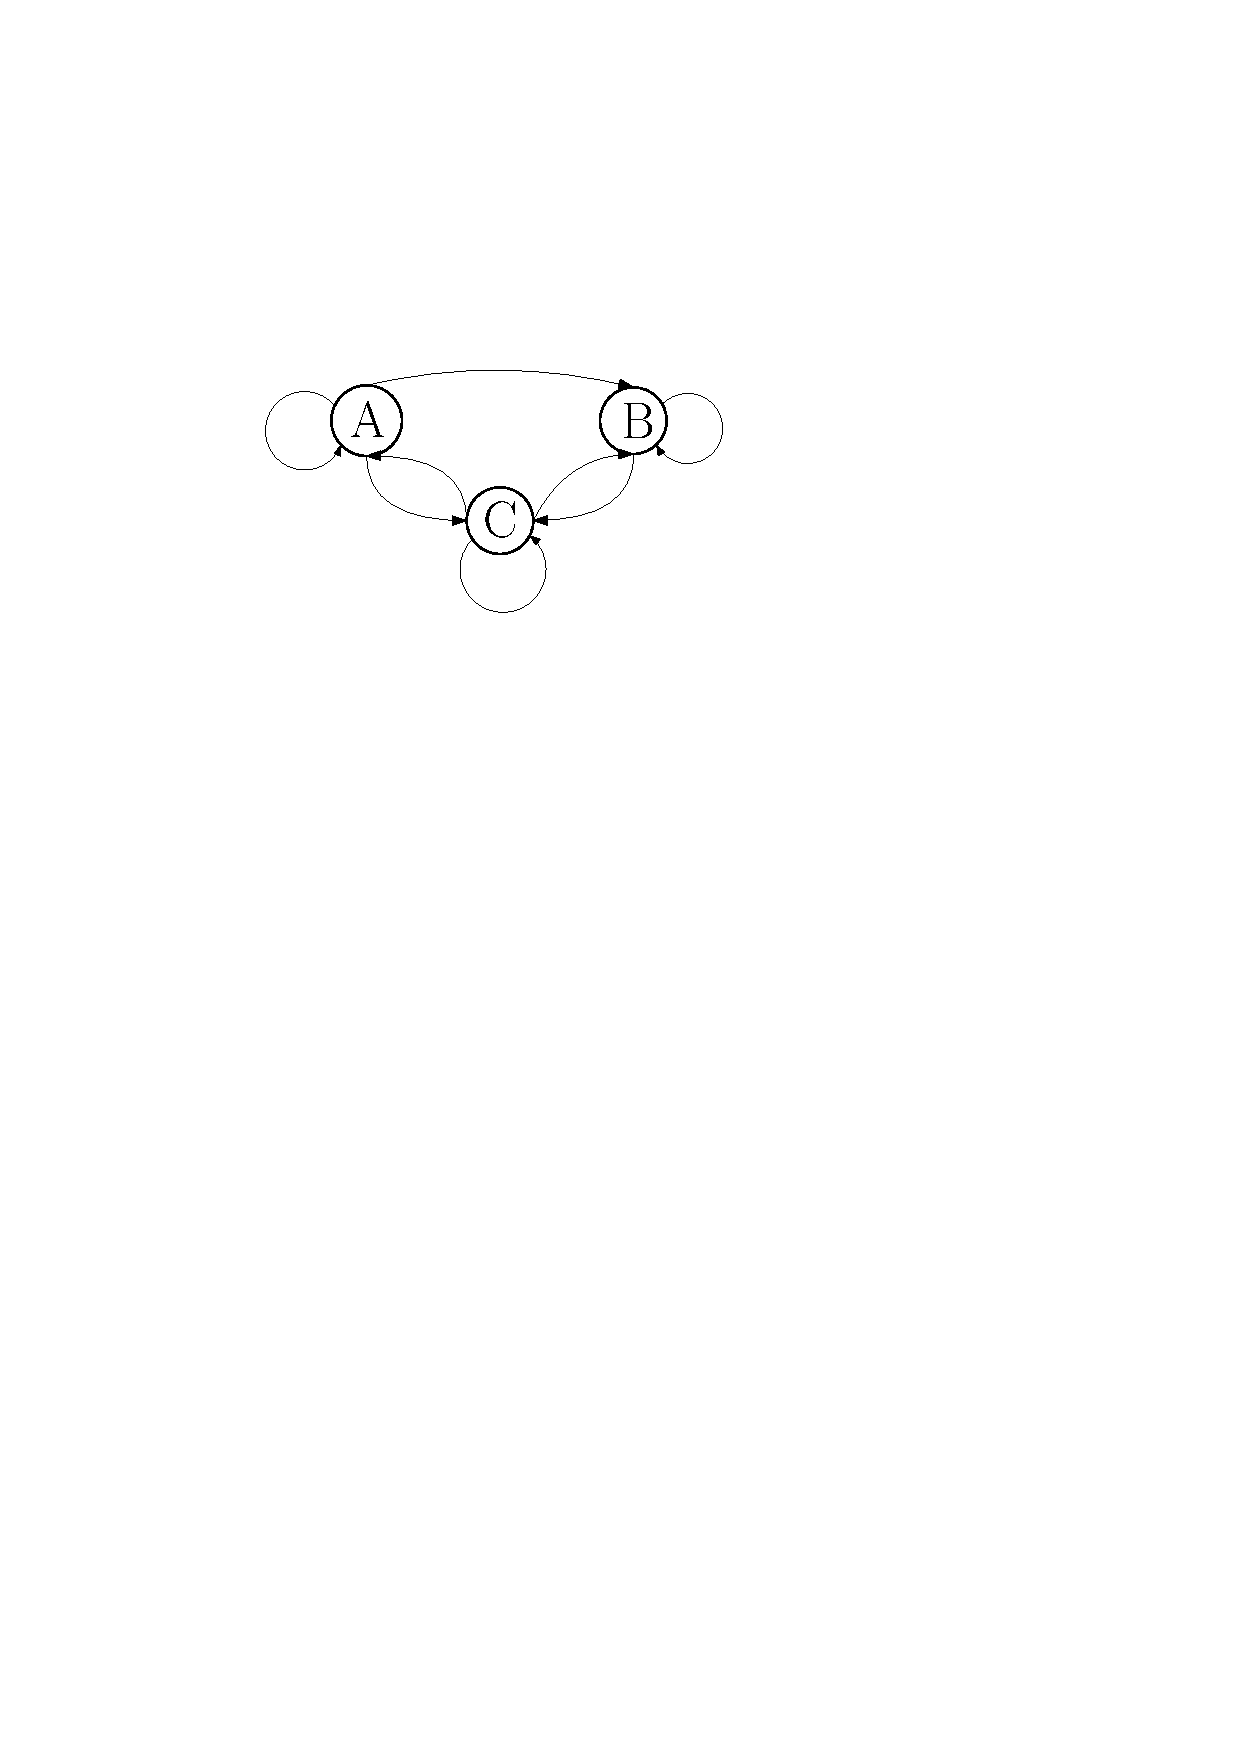
\includegraphics[width=1.0\textwidth]{../figures/chapter5/figures/markov_chain_irreducible.pdf}
	\caption[Illustration of an irreducible $3$-State Markov Chain]{An illustration of an irreducible $3$-State Markov chain.}
	\label{fig:app_markov_chain_irreducible}
\end{figure}

% Period of a Chain and Aperiodicity
A period of a state $x \in \mathcal{S}$ denoted as $d_x$ is defined for each state in the chain as follows \cite{Sokal1997},
\marginpar{period of a state}
\begin{equation}
	d_x = \text{GCD}\,\,\{n: p_{x,x}^{(n)} > 0, n > 0\}
\label{eq:app_markov_chain_period}
\end{equation}
where $\text{GCD}$ stands for the \emph{Greatest Common Divisor} of the set.

In an arbitrary discrete-state Markov chain, different states might have different periods.
\marginpar{periodic, aperiodic chain}
A state is called \emph{aperiodic} if its period is equal to $1$ and it is called \emph{periodic} otherwise.
If a chain has the same period $d > 1$ for each of its states then the chain is called \emph{periodic} (see Fig.~\ref{fig:app_markov_chain_periodic} for a periodic chain with period $3$).
A periodic chain exhibits a non-stochastic behavior in their dynamic.
On the contrary, a chain having the same period of $1$ for each of its states is called a \emph{aperiodic} chain (see Fig.~\ref{fig:app_markov_chain_aperiodic} for an example of a aperiodic chain).
\normdoublefigure[pos=tbhp,
                  mainlabel={fig:app_markov_chain_periodicity},
                  maincaption={Examples of periodic and aperiodic chains. (Left) an example of a periodic $3$-state Markov chain. In this case, all states have the the same period of $3$ iterations. (Right) an example of aperiodic $3$-state Markov chain, that is all states are aperiodic.},%
									mainshortcaption={Examples of periodic and aperiodic chains.},
                  leftopt={width=0.45\textwidth},
                  leftlabel={fig:app_markov_chain_periodic},
                  leftcaption={Periodic chain},
                  %leftshortcaption={},%
                  rightopt={width=0.45\textwidth},
                  rightlabel={fig:app_markov_chain_aperiodic},
                  rightcaption={Aperiodic chain},
                  %rightshortcaption={},
                  %spacing={\hfill}
                 ]
{../figures/chapter5/figures/markov_chain_periodic}
{../figures/chapter5/figures/markov_chain_aperiodic}

% Stationary Distribution
Some distributions are \emph{stationary} with respect to a transition probability matrix \cite{Sokal1997,Robert2004,Sargent2017}.
\marginpar{Stationary distribution}
Specifically, $\pi^*$ is \emph{stationary for} $P$ if,
\begin{equation}
	\pi^* = \pi^* P
\label{eq:app_markov_chain_stationary}
\end{equation}	
Put differently, the distribution is \emph{invariant} under transition.
Consequently, if stationary distribution exists,
once the chain reaches the stationary distribution, it will remain there and the chain itself becomes stationary. 
\marginpar{Stationary Markov chain}
Stationary distribution need not exist for a given $P$,
but in the application of \gls[hyper=false]{mcmc} algorithms,
the existence of stationary distribution is guaranteed \cite{Geyer2011}.

% Example of Stationary Distribution
As an example of a stationary distribution, consider once more the transition probability matrix $P$ in Eq.~(\ref{eq:app_transition_probability_matrix}).
For this transition, the distribution $\pi = [0.0, 0.0, 1.0]$ is stationary with respect to $P$ such that
\begin{equation}
	\pi = \pi P \Leftrightarrow [0.0, 0.0, 1.0] = [0.0, 0.0, 1.0] 		\begin{pmatrix}
		  0.75  & 0.20 & 0.05\\
      0.65  & 0.15 & 0.20\\
      0.00  & 0.00 & 1.00\\
		\end{pmatrix}
\label{eq:app_markov_chain_stationary_example}
\end{equation}
Stating that a stationary distribution is being dead, eventually and definitely.

% Markov Chain Convergence
The notions of irreducibility, aperiodicity, and stationarity are cobbled together to arrive at an important result in the discrete-state Markov chain and it is stated here without proof \cite{Sargent2017}.
\marginpar{Fundamental theorem of Markov chain}
Let $P$ be a transition probability matrix, irreducible and aperiodic, then $P$ has exactly one stationary distribution $\pi^*$ and for any initial distribution $\pi^{(0)}$
\begin{equation}
	\lim_{I \rightarrow \infty} |\pi^{(0)}P^I - \pi^*| = 0
\label{eq:app_markov_chain_convergence}
\end{equation}
That is, the chain converges \emph{in distribution} to the stationary distribution regardless of its initial distribution.
The theorem also indicates the existence of a \emph{limiting distribution} $\lim_{I \rightarrow \infty} \pi^{(0)}P^I$.

% Ergodic Theorem and convergence in probability
\marginpar{Ergodic theorem}
Furthermore, under the above condition,
\begin{equation}
	\lim_{I \rightarrow \infty} \frac{1}{I} \sum_{i=1}^{I} \mathbb{I}_{\{\mathcal{X}^{(i)} = x\}} = \pi_{x} \,\,\,\, \forall x \in \mathcal{S}
\label{eq:app_markov_chain_ergodic_theorem}
\end{equation}
where $\mathbb{I}$ is the indicator function where it is $1.0$ if the condition in the subscript holds, and $0$ otherwise.
In other words, the chain converges \emph{in probability}.
These theorems provide the justification for using samples generated from a Markov chain (whose properties stated above) as samples for Monte Carlo calculation.
For proofs of these theorems, refer to \cite{Robert2004}.

% Detailed Balance Condition
In generating samples from a target distribution, 
\marginpar{Detailed balance condition}
the engineering is done somewhat in reverse (``Given a distribution, construct $P$'').
Thus it is worthwhile to note the \emph{detailed balance} condition which is a central condition for an \gls[hyper=false]{mcmc} algorithm.
A Markov chain with a transition probability matrix $P$ satisfies the detailed balance condition if there exists a probability distribution $\pi$ such that,
\begin{equation}
  p_{x,y} \pi_x = p_{y,x} \pi_y \,\,\,\, \forall x,y \in \mathcal{S}
\label{eq:app_markov_chain_detailed_balance}
\end{equation}
\marginpar{Reversible chain}
As a result, the chain is said to be \emph{reversible}.
Formally,
\begin{equation}
  \mathcal{X}^{(i+1)}\,|\,\mathcal{X}^{(i)} = x \, \thicksim \, \mathcal{X}^{(i)}\,|\,\mathcal{X}^{(i+1)} = x \,\,\,\, \forall x \in \mathcal{S}
\label{eq:app_markov_chain_reversibility}
\end{equation}
A reversible chain is a stationary chain.
Consequently, in an \gls[hyper=false]{mcmc} algorithm,
if the transition probability satisfies the detailed balance condition with respect to the target distribution, 
it ensures the reversibility of the process and ultimately the stationarity of the chain.
Finally, imposing the conditions of irreducibility and aperiodicity, the stationary distribution of the chain converges to the target distribution.
For proof of this theorem see Refs.~\cite{Kelly1978,Robert2004}.
